\documentclass[10pt,a4paper,twocolumn]{article}
\usepackage[utf8x]{inputenc}
\usepackage{ucs}
\usepackage{amsmath}
\usepackage{amsfonts}
\usepackage{amssymb}
\usepackage{listings}
\usepackage{hyperref}
\usepackage{color}
\usepackage{graphicx} 
\definecolor{codebg}{rgb}{0.9,0.9,0.9}
\lstset{language=C++,
backgroundcolor=\color{codebg},
numbers=left,
xleftmargin=9pt,
framexleftmargin=9pt,
basicstyle=\scriptsize,
numberstyle=\scriptsize\color{black},
breaklines=true,
numbersep=1pt,
tabsize=2}
\newenvironment{quoteje} 
               { \noindent {\bfseries  "}}     
               {{\bfseries  "}\vspace{\parskip}}
\renewcommand\refname{References}
\author{Jeroen Heymans}
\title{Comparison of two object-oriented languages: C++ and Ruby}
\begin{document}
\maketitle

\tableofcontents

\section{Introduction}

\subsection{Foreword}
This paper is written for the master course Principles of Object Oriented Languages on the Vrije Universiteit Brussel. It contains a comparison of the object-oriented features from two languages that contain multiple object-oriented features. 

\subsection{The compared languages}
The choice for this paper was C++, a well-known static typed language with good object-oriented features, and Ruby, a dynamic typed language that was designed to be as object-oriented as possible.

\subsubsection{C++}
Originally called "C with classes", C++ is a multi-paradigm, static typed language based on the popular language C. C++ does not require you to write all code in an object-oriented fashion though, it is also possible to write all your code in a procedural way via functions. As a multi-paradigm language, it supports however many object-oriented features. We have tested all the C++ code in this paper with the GCC compiler on Ubuntu (version 4.5.2).

\subsubsection{Ruby}
When designing Ruby, the creator of Ruby, Ykihiro Matsumoto, looked at other languages to find an ideal syntax. He wanted a dynamic typed scripting language that was more powerful than Perl and more object-oriented than Python. In Ruby, everything is an object. It was influenced by Smalltalk, every type was given method instance variables. All Ruby code was tested with Ruby version 1.9.2p0 (2010-08-18 revision 29036).
\pagebreak

\section{Comparisons}

\subsection{Dynamic versus static typing}
C++ is a static typed language while Ruby is a dynamic typed language. Ruby supports duck typing which is credited to James Whitcomb Riley's words:

\begin{quote}When I see a bird that walks like a duck and swims like a duck and quacks like a duck, I call that bird a duck.\end{quote}

The type of a variable or object is determined at runtime.

Because of the difference in typing, there are some differences in Ruby and C++. For example, in C++ we can have multiple functions or methods with the same number of parameters but with other types. \textit{void foo(int)} and \textit{void foo(float)} are both different functions. In Ruby, this is not possible, only one function or method is allowed with the same name.

Due to the dynamic typed nature of Ruby, there is no need for constructions like templates in C++ to enforce one function or method to accept multiple types. Templates in C++ allow for creating generic functions, methods and classes. For example when we create a Stack class in Ruby, this can take any possible type of variable to put on the stack. 

In C++ however, because it is static typed, we need to notify upfront what the types of the elements on the stack will be. We could therefore write an \textit{IntegerStack}, \textit{FloatStack}, \textit{StringStack} and so on. With templates however, we can simply define a \textit{Stack\textless T\textgreater } where \textit{T} is the type that the stack will handle.

We must notify though that eventhough templates enable us to create a more generic version of a stack, this version is still not as generic as in Ruby. Because we still need to notify the type of the objects on the stack, we are limited to objects of this type. In Ruby, we can add anything we like on a stack without worrying that we combine strings, integers or other objects.

\subsection{Classes}
In object-oriented programming, a class is a blueprint that is used to construct objects. We call these constructed objects instances of a class. We compare the several types of classes that can be made in Ruby and C++.

\subsubsection{Abstract classes}
An abstract class is a class that can not be instantiated for it is either labelled as abstract or it specifies abstract methods. The general idea of abstract classes is that the class must be extended in order to gain access to the methods and members of the abstract class. In C++, an abstract class is a class having at least one pure virtual function. An example can be found in listing 1 in the appendix.

If we are trying to compile C++ code where we instantiate an abstract class, we will receive an error message from the compiler that notifies us that this operation is not allowed:

\begin{lstlisting}
g++ a.cpp -o a
a.cpp: In function 'int main()':
a.cpp:10:16: error: cannot allocate an object of abstract type 'A'
a.cpp:3:9: note: because the following virtual functions are pure within 'A':
a.cpp:5:16: note: virtual void A::f()
a.cpp:10:6: error: cannot declare variable 'a' to be of abstract type 'A'
a.cpp:3:9: note: since type 'A' has pure virtual functions
make: *** [a] Error 1
\end{lstlisting}

In order to use functionality defined in the abstract class, we need to inherit from the abstract class into another class where we override the virtual functions. If we do not override the virtual functions, the subclass will be an abstract class again.

Abstract classes in Ruby are a different story. Unlike some object-oriented languages, Ruby does not support a keyword like \textit{abstract} or a way like C++ to define an abstract class. Actually, Ruby does not provide the necessary standard tools to create abstract classes. However, the programmer himself can force a class to behave like an abstract class when he makes \textit{:new} (the constructor) private. The extending class must then make \textit{:new} public. This way, as long as there is no class that extends the class A with a private constructor, the methods in A will never be accesible as it is not possible to construct an instance of A, thus it behaves like an abstract class. The example code can be found in listing 2 in the appendix.

\subsubsection{Final classes}
A final class is a class that can not be extended. This could be done for reasons of security and efficiency. Final classes are not supported in C++ nor Ruby. However, there exist mechanisms to prevent programmers from extending other classes. An example of such a mechanism in C++ can be found in listing 3 of the appendix.

In this example, we made the class named Final final. We did this by creating a class Final that inherits from the class MakeFinal. In class MakeFinal, we have a private constructor which can only be called by the class Final as the class Final is marked as \textit{friend}. By inheriting MakeFinal \textit{virtual} in the class Final, we make sure that the constructor \textit{MakeFinal()} must be called if we derive the class Final. As only Final is a friend, this will generate a compile error that notifies us that \textit{MakeFinal()} is private if we would try to create an instance of MakeFinal. Via this mechanism, we have ensured that the class named Final is really final. 

In Ruby, we can create a similar mechanism as can be found in listing 4 of the appendix. In this example, we add a method \textit{final} to the standardclass \textit{Class}. In this method \textit{final}, we define that a new method called \textit{inherited} should be added to the class given by the parameter \textit{klass}. If we then add a call to \textit{final} to our own defined class, the code for the method \textit{inherited} will be injected in our own class. \textit{inherited} is a method that will always be called whenever we try to inherit the class that contains this method. In our example, this will cause a \textit{RuntimeError}, thus disallowing the programmer to continue programming as long as we try to inherit from our \textit{final} class.

But is a class really final in Ruby? Not even if we force a class to be marked as final like we did in the example? Unfortunately not. This is due to the \textit{open classes} concept of Ruby that will always allow you to add methods to a class, whether it is marked as \textit{final} like in our example or not. See the section "Partial classes" however for an example on how to prevent extending an open class.

\subsubsection{Friend classes}
C++ has an unique keyword: \textit{friend}. With this, one can declare a class as a friend:

\begin{lstlisting}
class A;
class B {
	friend class A;
}
\end{lstlisting}

In this example, class A is a friend of B. This means that class A has more access rights to the members and methods of class B. More concrete, this means that all private and protected members and methods of B are accessible by A while this would not be the case by default. The \textit{friend} keyword defines the following features:

\begin{itemize}
\item Friendships are not corresponded: if class A is a friend of class B, class B is not automatically a friend of class A.
\item Friendships are not transitive: if class A is a friend of class B and class B is a friend of class C, then is class A not a friend of class C.
\item Friendships are not inherited: if there is a class Base with a friend, then the class Derived (that inherits from Base) does not have that same friend. The same goes up for all friends of Derived, they are not automatically friends of Base. The same goes in the other direction: if Base (or Derived) is a friend of a class, then is Derived (or Base) not automatically a friend of the same class.
\item The restricted members and methods from Base that are inherited by Derived are accessible by a friend class of Derived if Derived itself can access these members and methods. So if Derived inherits publicly\footnote{See the section "Derived classes" in "Access control" for more details on deriving classes.} from Base, Derived only has access to the protected and public members from Base, not the private members, so neither does a friend (the same goes for methods).
\end{itemize}

Friend classes are not possible in standard Ruby, however there exist some libraries\footnote{An example can be found on https://github.com/lsegal/friend} that allow a programmer to define friend classes in Ruby.

\subsubsection{Inner classes}
Inner classes are called nested classes in Ruby. They can simply be defined like you would expect, by simply putting a class definition within a class definition as you can see in listing 6 in the appendix. If we have a class A with an inner class B, we can construct an object of the type \textit{A} for the outer class and \textit{A::B} for the inner class:

\begin{lstlisting}[language=Ruby]
b = A::B.new
a = A.new
\end{lstlisting}

With the \textit{::} operator in \textit{A::B}, we simply say: "Take class B that is defined inside the scope of A". The object of class B can be treated like it was never defined in A. Both instances of the classes can exist completely on their own: if you make an instance of A, this will not indirectly create an instance of B and vice-versa. This means that an instance of B will not have access to the methods and members of A, only to the methods and members of its own instance. The same goes for an instance of A. Only if there is an explicit construction of an object B or A in respectively A or B, they will be able to access the methods and members.

With inner classes in C++, almost the same story exists. In order to access data from the inner class via the outer class or from the outer class via the inner class, an instance must be present to access this data. This can be achieved when constructing the inner or outer class as can be seen in listing 5 in the appendix.

Let us explain the code. What we have here are two classes: A as an outer class and B as an inner class. Upon construction of A, we automatically call the constructor of B with an instance of A. With this, B has a pointer that points to the object of A. A itself remembers the pointer to B that has been constructed. With this, it is possible to access A from within B and B from within A. Similar code can be written for Ruby where we also construct an instance of class A in class B and vice-versa.

However, there are some rules concerning the access to and from the inner class in C++. The code from the listing will compile and work. But if you look closely, the method \textit{f()} from the class B can access member \textit{a} from class A eventhough \textit{a} is defined as private. So in fact, the inner class gets the privilege to act as if it is part of the outer class.

We must notice though that there is a different story when you want to access the inner class. In the code, A has a method \textit{f()} that can access the member \textit{test} that is defined in B, via the pointer to B that was saved in A. This is because the member \textit{test} is defined as \textit{public}. If we however define \textit{test} as \textit{protected} or \textit{private}, the compiler will notify us that this is not allowed.

We can therefore conclude that an inner class in C++ gets the privilege to access everything from its outer class, even the private and protected members or methods. This is in contrast to how the outer class can access the inner class, in this case the standard access rules are applied. In Ruby, there are no special access rights for inner and outer classes, the standard rules are applied as enforced by the access specifiers \textit{public}, \textit{protected} and \textit{private}.

\subsubsection{Metaclasses}
For every defined class in Ruby, there exists a metaclass. For example if we define a class Person, Ruby automatically creates a metaclass MetaPerson\footnote{Internally a class for X will not be called MetaX but we want to make it more readable.}. The role of the metaclass MetaPerson is to split behaviour between Class (to create new classes) and class specific behaviour.

Ruby has two different types of methods: class methods and instance methods. Class methods are not designed to work on a specific instance of the class while instance methods are specifically designed to work on an instance of the class. Class methods are often compared to what we call static methods in other languages while instance methods can be compared to normal methods in other languages. The class methods are saved in the metaclass of the class. The class methods of Person are in fact instance methods of MetaPerson.

The same goes up for class variables and instance variables. Class variables are comparable to static variables in other languages: they are not instance-specific while instance variables are instance-specific. The class variables of Person are in fact instance variables of MetaPerson.

C++ does not have built-in support for metaclasses.

\subsubsection{Partial classes}
A partial class is a class whose definition may be splitted into multiple pieces. These pieces can be within one source file or across multiple files. Ruby supports the notion of partial classes. With this, it is possible to extend existing classes with new methods or members. Its not necessary that the class is user-defined, it can be for example the built-in \textit{String} class as you can see in listing 7 in the appendix. The result of executing \textit{doublePrint} on a String object, will give as a result: "\textit{testtest}".

Partial classes like in Ruby, do not exist in C++. It is not possible to add new methods or members on-the-fly. The reason for this is that Ruby classes are considered "open" while C++ classes are "closed". When you define a C++ class in the typical header-file, there is no possibility to split this definition in several files, e.g. multiple header files for the same class are not allowed. Only the definition of the methods themselves can be split over mutiple source-files. It is for example possible to have a header-file "a.h" and multiple source-files like "method1-from-a.cpp" and "method2-from-a.cpp". Still, this does not create pure open classes like in Ruby where you can add methods at runtime, it is merely a way to make smaller files.

If you do not want that classes are further extended in Ruby, then the possibility of \textit{freezing} the class exists. By simple adding the keyword \textit{freeze} to the class, you declare the class as frozen (e.g. not modifiable). From then on, the class is considered as \textit{closed} instead of the default \textit{open}. Classes in C++ could be regarded as standardly \textit{frozen}.

\subsection{Access control}

\subsubsection{Access control on members and methods}
C++ offers three keywords that define access control on members and methods of classes: \textit{public}, \textit{protected} or \textit{private}. 

\begin{itemize}
\item \textit{public}: the member/method is accessible without any restriction
\item \textit{protected}: only the class that defines the member/method, the friend classes of the class and the subclasses of the class can access the member/method
\item \textit{private}: only the class that defines the member/method and the friend classes of the class can access the member/method
\end{itemize}

Ruby also provides these three keywords but there are some subtle differences. The difference between Ruby and C++ can be found in the objects on which a private method is called or a private member is requested. The C++ code that explains this can be found in listing 8 in the appendix and the Ruby code in listing 9 in the appendix. As you can see, we have a class A in which the \textit{test()}-method accepts a parameter to an A object. All three calls to the method \textit{foo()} work: with an implicit receiver and an explicit receiver like \textit{this} or \textit{a}. We can conclude that in C++, it is possible to access private members and methods from an object, as long as it is the type of object as where the actual calls are done. 

If we try the Ruby equivalent of this code, we get into trouble. Both the lines \textit{self.foo} and \textit{obj.foo} generate the same error: \textit{NoMethodError}. This is because we use an explicit receiver. If you want to access a private member or method in Ruby, you can only use an implicit receiver. With any explicit receiver, even if that is \textit{self}, the \textit{NoMethodError} will be generated. We can conclude that Ruby depends on the type of the receiver if it will give you access to a private member or not. Only with an implicit receiver will you gain access to private members or methods, even if the explicit receiver is \textit{self}.

In C++, this distinction does not exist. As long as you try to access the private member or method from code that is defined in the private member or method of his class, everything is okay. So if we have a private member \textit{test} in a class A, we can even access that member via an object instantiated from A that is not equal to \textit{this}, as long as the code is placed in the body of class A. Note: we have seen in the section "Friend classes" that friends of a class also have access to the private members and methods from a class.

\subsubsection{Derived classes}
When declaring a derived class in C++, we can provide an access specifier: \textit{public}, \textit{protected} or \textit{private}. For example if we have the base class A, we can create subclass B from A and provide one of the three access specifiers \textit{public}, \textit{protected} or \textit{private} like this:

\begin{lstlisting}
class A { };
class B: public A { };
class C: protected A { };
class D: private A { };
\end{lstlisting}

The purpose of this access specifier is to alter the access control of the members of the base class via the derived class. The access control is not altered on the original base class, only on the derived class. For example, if we derive a class as private, this does not mean that the methods and members of the original class become private, they keep their access specifier. If you want however to access a public member or method from a superclass via a subclass instance that was derived as private, you will receive an error. For an exmple, see listing 10 of the appendix.

When deriving a class in C++, the following situations can occur:
\begin{itemize}
\item Derive as \textit{public}: public and protected members of the base class remain public and protected members of the derived class.
\item Derive as \textit{protected}: public and protected members of the base class become protected members of the derived class.
\item Derive as \textit{private}: public and protected members of the base class become private members of the derived class.
\end{itemize}

In all cases, private members of the base class remain private, e.g.: not even the derived class can access them unless there is a specific friend declaration within the base class that explicitly grants access to them. If we do not provide an access specifier, the access rules of the baseclass are simply copied, e.g.: public remains public, protected remains protected.

Unlike C++, Ruby does not support the changing of the access properties of members and methods of the superclass via one keyword when we derive a class. This has to be done individually for every member or method.

We notice though, Ruby has the strange property to allow the call to private methods and members from the superclass via the subclass. An example:

\begin{lstlisting}[language=Ruby]
class Animal
	private
	def speak
		puts "Random noise"
	end
end

class Cat < Animal
	public
	def speak
		super
	end
end
\end{lstlisting}

When we excecute the following code:

\begin{lstlisting}[language=Ruby]
cat = Cat.new
cat.speak
\end{lstlisting}

This will print \textit{Random noise}. The explanation behind this is that Ruby actually allows to call private methods and members from a class via an implicit receiver. If you use an explicit receiver (for example \textit{Animal.speak}) the call will fail like you would expect. So although Ruby does not have an access specifier when deriving a class, it is however possible to mimic the behaviour from C++, even with more detail as you can enable the access to private members and methods of the superclass. Ofcourse, overriding a method or member with a different access specifier is possible in C++. In case of a method, you have to call the superclass method with an explicit receiver. It is however not possible to gain access to private members or methods from the superclass, even by overriding the corresponding member or method.

\subsection{Inheritance}
In Ruby, a class can only inherit from a single other class. Some other languages like C++ support multiple inheritance, a feature that allows classes to inherit features from multiple classes.

We can define a superclass Animal and a subclass Cat in Ruby like we did in the listing number 11 in the appendix. When using these two classes, one can see that methods will be overriden:

\begin{lstlisting}[language=Ruby]
cat = Cat.new
cat.speak
cat.breath
\end{lstlisting}

This will output:

\begin{lstlisting}
Random noise
Breathe
\end{lstlisting}

This is classical single inheritance. C++ however supports multiple inheritance. With multiple inheritance it is possible to inherit from multiple classes like this:

\begin{lstlisting}
class C: public A, protected B { };
\end{lstlisting}

In this example, a class C is created that inherits publicly from class A and protectedly from class B. As you can see, the access modifiers can be different. 

One of the common pitfalls when using multiple inheritance in C++ is ambiguities:

\begin{lstlisting}
class A { virtual void f(); };
class B { virtual void f(); };
class C : public A ,public B { void f(); };
\end{lstlisting}

This issue can be solved by using explicit qualification. We explicitly tell the compiler which \textit{f()} we would like to call:

\begin{lstlisting}
C* c = new C;
c->f();
c->A::f(); // call f() from class A
c->B::f(); // call f() from class B
\end{lstlisting}

Because of multiple inheritance, C++ does not support the keyword \textit{super} which makes it possible to call methods and retrieve members from the superclass. If you inherit from class A and class B, to which class should \textit{super} point? To avoid confusion and get clear code, one always has to use explicit qualification when calling the superclass.

\begin{figure}
\caption{The diamond problem}
\begin{center}
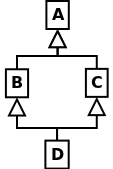
\includegraphics[scale=0.6]{diamond.png}
\end{center}
\end{figure}

Another more complex problem which can arise with multiple inheritance is called the \textit{diamond problem}. The diamond problem is an ambiguity that arises when two classes B and C inherit from A, and class D inherits from both B and C. If a method in D calls a method that is defined in A (and D does not override the method) and B and C have overridden that method differently, then from which class does it inherit: B or C? This is a problem that can be solved by using virtual inheritance.

When constructing an object of class D, C++ actually creates in the memory objects of B and C internally. B and C in their turn also construct each an object of A. This means that upon the creation of D, 4 internal objects are created: B, C and 2 times A. If we however have inherited B and C from A as virtual (for example: \textit{class B: virtual public A}), C++ will make sure that only one object of A is constructed. Since there is only one object of A, we now only have one possible method that was defined in A. If we want to access the methods from B or C, we simply have to prefix with respectively \textit{B::} or \textit{C::}.

Although Ruby does not support multiple inheritance, it eliminates the need for multiple inheritance by providing mixins. As a programmer, you can define modules in Ruby. In classes, you can then include these modules. For example:

\begin{lstlisting}[language=Ruby]
module Foo
	def Bar
		puts "Wazaa!"
	end
end

class FooBar
	include Foo
end
\end{lstlisting}

In this example, the class FooBar contains the content of module Foo (in this case the method Bar). It is possible to include multiple modules, even if the modules contain the same methods as you can see in listing x in the appendix.

Our code from listing x in the appendix will output "\textit{Module B}". The order in which a programmer includes modules, depends on what methods will be available. If we would have included A after B, the output would be \textit{Module A}. As modules are included, they override functionality that was defined in the lines before the include. Methods that are defined after the include statement, will override methods that were included.

\subsection{Polymorphism}
The literal meaning of polymorphism is "the ability to take on multiple forms or shapes". This refers, in a broader sense, to the ability of different objects to respond in different ways to the same message or method invocation. We have written an example in Ruby that shows what polymorphism can do, see listing 13 in the appendix. In our example, we see that the classes Dog and Cat are subclasses from Animal. We create a Dog and Cat object and call the method \textit{makeNoise}. The output is correctly:

\begin{lstlisting}[language=Ruby]
Woof!
Meow!
\end{lstlisting}

Even though Cat and Dog are different classes, they implement the same messages with a different implementation but can be called in exactly the same way. Via the implementation of \textit{makeNoise} in the class Animal, we make sure that there will be a clean error when someone has subclassed Animal but not overwritten \textit{makeNoise}; thus ensuring that all the subclasses of Animal understand the same message \textit{makeNoise} but with their own implementation. An equivalent example in C++ code can be found in listing 12 in the appendix. This code correctly outputs: 

\begin{lstlisting}[language=Ruby]
Woof!
Meow!
\end{lstlisting}

As you can see, we treat the objects Dog and Cat like they were Animal objects. We call the same method \textit{makeNoise()} on an object that needs to be an Animal object. This results in different results, e.g.: the same message results in a different execution that is based on the actual type of the object.

Because Ruby is a duck typed language, it is even possible to disable the need for subclassing from the class Animal. It is perfectly possible to implement a class Car that is not subclassed from Animal and has a method called \textit{makeNoise} which results in printing "vroom". We can pass an instance of Car to the method print and it will work. The reason behind this, is that there is no real type checking in the background.

\begin{quote}
When I see a bird that walks like a duck and swims like a duck and quacks like a duck, I call that bird a duck.
\end{quote}

As long as the parameter of \textit{print} is an object that has a method \textit{makeNoise}, the interpreter of Ruby will not complain.

Such a system like in Ruby, can be simulated via the use of templates. With templates, you can for example make generic functions. If we take the example of a Cat and a Dog, we can modify the code so the \textit{print} function does not longer require that his only parameter is a pointer to an Animal-object. You can find the code in listing 14 in the appendix. By parameterizing this, we can enable the possibility to give an instance of the class Car to the print-function. This will work correctly as long as the given object has the methods that are called and the members that are requested or modified in the body of the templated function.

\subsection{Namespaces/modules}
Namespaces in C++ are a method to group classes, functions and other identifiers in one block. An example can be found in listing 15 in the appendix. Outside the block of a namespace, one must prefix the identifiers he wants to access with the namespace specifier. If you look at our example, if we want to access the integer \textit{test} that was defined within the namespace A, we need to prefix with \textit{A::} so we get: \textit{A::test}. To ommit the prefixing, one can use the following statement:

\begin{lstlisting}
using namespace abc;
\end{lstlisting}

With this line, it is no longer necessary to prefix with \textit{abc::}. Namespaces are hierarchical, there can be mutiple namespaces defined in another namespace. When requesting an identifier in the code in a namespace, the compiler start searching from the namespace where the identifier is requested. For example if we request C in code that is put in A::B, the compiler will first search if there exists a C in A::B. If not, the compiler searches in A and after that in the global namespace.

Modules are the Ruby equivalent of namespaces, an example can be found in listing 16 in the appendix. They can also be defined hierarchical. The difference with C++ namespaces is that modules can be included in classes. This allows programmers to add new methods to classes. If several classes implement exact the same method, this method can be placed in a module to ensure that every class has the same code. This concept is called mixins which is an alternative in Ruby to multiple inheritance in C++. It is discussed more in the section "Inheritance".

\subsection{Reflection}
In standard C++, reflection is not possible. The popular framework Qt has however implemented reflection features\footnote{A class that is important to have reflection in Qt is for example QMetaObject: http://doc.qt.nokia.com/5.0-snapshot/qmetaobject.html}.

Reflection is possible in Ruby. Via several standard methods, we get lots of possiblities in Ruby to perform reflection-related operations:

\begin{itemize}
\item Instance variables: setting, getting and removing
\item Class variables: setting, getting and removing
\item Methods: define, undefine, alias
\end{itemize}

Define, undefine and alias of methods can be done on instance methods and class methods. To perform these operations on instance methods, we must work on an instance of a class. If we want to perform these operations on class methods, we must work on the metaclass.

When performing reflection, the rules defined via the access specifiers \textit{public}, \textit{protected} and \textit{private} are completely ignored. With reflection, it is therefore for example possible to get private members of an instance.

\subsection{Interfaces}

Both C++ and Ruby do not support a keyword like \textit{interface}. It is however possible to enforce interfaces in these languages. In C++ this is done very easily: create an abstract class that only consists of virtual functions without a body, such a class is equivalent to an interface. This enforces inherited classes to implement all the methods. If an inherited class only implements a few of the virtual functions thus not all of them, the inherited class will be an abstract class. An example of this can be found in listing x in the appendix.

Via several modules, one can enforce interfaces in Ruby\footnote{An example of an implementation of interfaces can be found on http://www.metabates.com/2011/02/07/building-interfaces-and-abstract-classes-in-ruby/}. Generally, it is the same story as with abstract classes in Ruby but you enforce the programmer to override all the methods of a class.

\subsection{Method overloading}

C++ supports method overloading. It is possible to define multiple methods with the same name but with another arity or other types for the parameters. When compiling, the compiler will determine which method will be called during runtime.

Because Ruby is a dynamic typed language, method overloading is not possible.

\subsection{Constructors}

Constructors in C++ must have the name of the class as their name. If you want to define a constructor in the class \textit{Foo}, the constructor must be named \textit{Foo()}. Due to method overloading, it is possible to define more constructors where the types of the parameters or the arity may defer. Standardly, a compiler will make sure that there is a standard constructor in the class that accepts no arguments. 

In Ruby, the constructor of a class is called \textit{initialize}. Due to the lack of method overloading, it is not possible to define more than one constructor in a class. Constructors in Ruby are inherited. If you look at listing x in the appendix, you can see that the constructor of class \textit{Foo} is also avaiable for class \textit{Bar} because \textit{Bar} is an inherited class of \textit{Foo}.

We must note that constructors in C++ are not inherited like in Ruby. For example, if we have a class \textit{Foo} with a constructor that takes on argument (for example \textit{Foo(int)}) and we define a subclass of \textit{Foo} called \textit{Bar}, we cannot construct on object via \textit{Bar(int)} unless we define it explicitely. Constructors must be rewritten in derived classes if you want them to be usable.

\subsection{Destructors}

Natively, Ruby does not support destructors. It however offers something similar called \textit{ObjectSpace.define\_ finalizer}\footnote{Can be found on http://www.ruby-doc.org/core-1.9.3/ObjectSpace.html\# M001527}. With this, it is possible to define what must happen when an object will be collected by the garbage collector.

C++ natively supports destructors. They are always noted as \textit{\~NameOfClass()}. Destructors never accept parameters and cannot return data. They are implicitly called when an object passes out of scope, unless this object was defined as \textit{static} or \textit{extern}. A programmer can also invoke destructors explicitly by using the \textit{delete} operator. For example, if we have an object created via \textit{A* foo = new A();}, we can invoke the destructor of the object \textit{foo} by calling \textit{delete foo}.

\subsection{Everything is an object?} 

One of the main features of Ruby is the fact that everything is an object, even primitive types like an integer. Ruby follows the influence of the Smalltalk language by giving methods and instance variables to all of its types. An example of this feature:

\begin{lstlisting}[language=Ruby]
5.times { print "test".length }
\end{lstlisting}

This will generate the output: \textit{44444}. What it does is take an object \textit{5} of the type Number, call the method \textit{times} on it so it excecutes five times the part between { and }. The code \textit{print "test".length} will be excecuted five times which is effectively printing the length of the String object "test".

In C++, not everything acts as an object. The primitive data types: \textit{char}, \textit{short}, \textit{int}, \textit{long}, \textit{bool}, \textit{float}, \textit{double}, \textit{long double} and \textit{wchar\_t} ; do not have a class that provides methods to call on the data types. The data type \textit{string} is an exception to this as it does have its own class that can be used when including the library \textit{string}.

\section{Conclusion}
Ruby was designed to be as object-oriented as possible. Everything had to be an object. Eventhough this is correctly implemented, there are quite some differences with the object-oriented features that are provided by C++. The abscence of certain keywords do not allow features like for example friend classes. Though, most of these features that are not standard available in Ruby, can be implemented by clever use of modules and method implementations.

Does the abscence of certain features make Ruby less object-oriented than C++? Not at all, there is just a difference between the audiences of both languages. C++ is more low-level than Ruby which is why concepts as "everything is an object" and reflection are most of the time obsolete in C++. This is because these concepts make the code possibly more memory-consuming or the program more dynamic than one needs.

Both languages are equipped with a good basis for object-oriented programs, they simply have other implementations basic of the difference in audiences.

\section{References}
\begin{enumerate}
\item \url{http://www.ruby-lang.org/en/about/}
\item \url{http://www.cplusplus.com/info/history/}
\item \url{http://publib.boulder.ibm.com/infocenter/lnxpcomp/v8v101/index.jsp?topic=\%2Fcom.ibm.xlcpp8l.doc\%2Flanguage\%2Fref\%2Fcplr142.htm}
\item \url{http://www.klankboomklang.com/2007/10/05/the-metaclass/}
\item \url{http://ruby-extra.rubyforge.org/classes/Object.html}
\item \url{http://www.wikyblog.com/AmanKing/Metaclass_in_Ruby}
\item \url{http://www.klankboomklang.com/2007/10/12/objects-classes-and-jruby-internals/}
\item \url{http://shiningthrough.co.uk/A-comparison-of-Ruby-pass-by-reference-and-C++-pass-by-reference}
\item \url{http://rubylearning.com/satishtalim/ruby_inheritance.html}
\item \url{http://publib.boulder.ibm.com/infocenter/lnxpcomp/v8v101/index.jsp?topic=\%2Fcom.ibm.xlcpp8l.doc\%2Flanguage\%2Fref\%2Fcplr130.htm}
\item \url{http://www.skorks.com/2010/04/ruby-access-control-are-private-and-protected-methods-only-a-guideline/}
\item \url{http://weblog.jamisbuck.org/2007/2/23/method-visibility-in-ruby}
\item \url{http://stackoverflow.com/questions/137661/how-do-you-do-polymorphism-in-ruby}
\item \url{http://www.cplusplus.com/doc/tutorial/variables/}
\item \url{http://www.brpreiss.com/books/opus8/html/page597.html}
\item \url{http://www.java2s.com/Code/Ruby/Class/classvariablevsobjectvariable.htm}
\item \url{http://cplusplus.co.il/2009/09/01/final-frozen-classes-in-cpp/}
\item \url{http://www.geeksforgeeks.org/archives/16222}
\item \url{http://www.metabates.com/2011/02/07/building-interfaces-and-abstract-classes-in-ruby/}
\item \url{http://publib.boulder.ibm.com/infocenter/lnxpcomp/v8v101/index.jsp?topic=\%2Fcom.ibm.xlcpp8l.doc\%2Flanguage\%2Fref\%2Fcplr380.htm}
\end{enumerate}

\pagebreak
\section{Appendix}
\lstinputlisting[language=C++,caption={Abstract classes in C++}]{cpp/classes-abstract.cpp}
\lstinputlisting[language=Ruby,caption={Abstract classes in Ruby}]{ruby/class-abstract.rb}
\lstinputlisting[language=C++,caption={Final classes in C++}]{cpp/classes-final.cpp}
\lstinputlisting[language=Ruby,caption={Final classes in Ruby}]{ruby/class-final.rb}
\lstinputlisting[language=C++,caption={Inner classes in C++}]{cpp/classes-inner.cpp}
\lstinputlisting[language=Ruby,caption={Inner classes in Ruby}]{ruby/class-inner.rb}
\lstinputlisting[language=Ruby,caption={Partial classes in Ruby}]{ruby/class-partial.rb}
\lstinputlisting[language=C++,caption={Access control in C++: the use of implicit/explicit receivers}]{cpp/classes-access-control.cpp}
\lstinputlisting[language=Ruby,caption={Access control in Ruby: the use of implicit/explicit receivers}]{ruby/class-access-control.rb}
\lstinputlisting[language=C++,caption={Derived access control in C++}]{cpp/classes-access-control-derived.cpp}
\lstinputlisting[language=Ruby,caption={Inheritance in Ruby}]{ruby/class-inheritance.rb}
\lstinputlisting[language=C++,caption={Polymorphism in C++}]{cpp/classes-polymorphism.cpp}
\lstinputlisting[language=Ruby,caption={Polymorphism in Ruby}]{ruby/class-polymorphism.rb}
\lstinputlisting[language=C++,caption={Templates in C++}]{cpp/classes-template.cpp}
\lstinputlisting[language=C++,caption={Namespaces in C++}]{cpp/classes-namespace.cpp}
\lstinputlisting[language=Ruby,caption={Modules in Ruby}]{ruby/class-module.rb}

\end{document}
